\section{Verschlüsselung unter iOS}
	In diesem Kapitel werden die Kryptographie von iOS genauer vor gestellt.
	Dazu werde ich erst auf eingesetzt Hardware eingehen und dann auf die logische
	Ebene wechseln mit einem Fokus auf Dateizugriff.
	\subsection{Kryptographische Hardware}\label{sec:crypto-engine}
		Für eine native Verschlüsselung sorgt in jedem iOS Gerät eine AES256 bit
		basierte Hardware-Engine, welche zwischem dem Flash	Speicher und dem
		Systemspeicher liegt. Diese Positionierung sorgt für hohe Performance und
		niedrige Latenzen beim Verschlüsseln von Dateien. Die geräteeigene Unique ID
		(UID) wird beim Herstellungsprozess in den Applikationsprozessor und den Secure
		Enclave eingebrannt und die Group ID (GID) wird compiliert, somit ist es keiner
		Soft- oder Firmware möglich diese direkt zu lesen. Dies verhindert eine
		Manipulation oder ein Umgehen dieser Schlüssel, sowie einen Zugriff außerhalb
		der Krypto-Engine. Die UID erlaubt außerdem eine Gerätspezifische Bindung von
		Daten.
		Apple beteuert unter anderem
		\begin{quote}
			The UIDs are unique to each device and are not recorded by Apple or any of its
			suppliers.\cite[S.9]{iOSSecurityApr2015}
		\end{quote}
		Die GID hingegen ist allen Geräten einer Prozessorklasse bekannt, z.B. all
		jenen die einen Apple A7 nutzen. Dies liegt an der weniger
		Sicherheitskritischen Nutzung dieser Schlüssel für Vorgänge,
		wie beispielsweise die Übertragung von System Software bei Updates. Jegliche
		weitere bei Kryptografischen Operationen benötigte Schlüssel werden von einem
		Random Number Generator (RNG) mit einem auf	CTR\_DRBG\cite{NISTDRBG2012}
		basierendem Algorithmus erzeugt.
	\subsection{Schutz auf Dateiebene}
		Zusätzlich zur Hardwareverschlüsselung nutzt iOS ein Feature namens \textsl{Data
		Protection} um Daten auf dem Flash Speicher zu schützen. Dieser Mechanismus
		wird bei allen System Apps und ab iOS7 auch bei Drittanbieter Apps
		automatisch angewendet. Die Funktionsweise ist Form einer Schlüsselhierarchie
		im Verbund mit Hardwareverschlüsselung realisiert. Jede Datei, die in den
		Speicher geschrieben wird, erhält einen 256 Bit explizit ihr zugewiesenen
		\textsl{Per-File} Schlüssel. Dieser wird von der
		%TODO: get infos about AES-CBC + the initialization vector
		Verschlüsselungsengine (siehe: \ref{sec:crypto-engine}) mit Hilfe von
		AES Cipher Block Chaining verschlüsselt. Der Per-File Schlüssel wird mit
		einem von vier Klassenschlüsseln ummantelt und in den Meta-Daten gespeichert.
		Der Klassenschlüssel ist zusätzlich noch mit der UID und für manche auch mit
		dem Passcode des Benutzer gesichert. Jegliche Meta-Daten sind mit einem
		zufälligen Schlüssel verschlüsselt, welcher beim installieren von iOS oder
		beim Löschen eines Gerätes durch den Benutzer erstellt wird. Beim
		Entschlüsseln einer Datei, werden zuerst die Meta-Daten mit dem \textsl{File
		System Key} entschlüsselt. Dieser ist im \textsl{Effaceable Storage}
		gespeichert - einem dedizierten Bereich im NAND-Speicher, welcher direkt
		adressiert und sicher gelöscht werden kann.
		Sobald dieser Speicher und somit der darin enthaltene Dateisystem Schlüssel
		gelöscht wurde, macht dies alle Dateien auf dem Gerät kryptografisch
		unwiederherstellbar. Sobald der Benutzer einen Passcode auf dem System
		einrichtet, aktiviert er Data Protection.
		\begin{figure}[h]
			\centering
			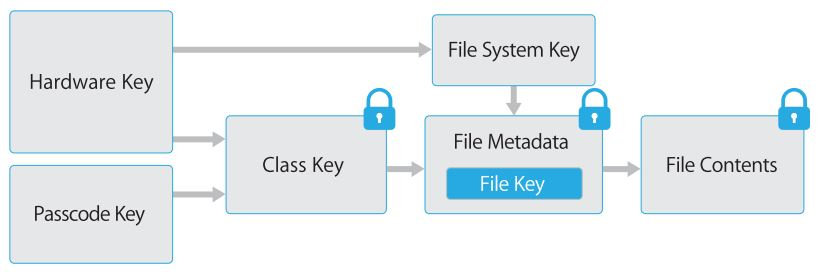
\includegraphics[width=0.9\linewidth]{ios/media/data-protection.jpg}
			\caption{Data Protection Architektur 
			\cite[S.10]{iOSSecurityApr2015}}
			\label{fig:data-protection}
		\end{figure}
